\subsection{The Periodic Table}
Source: \href{https://www.youtube.com/watch?v=0RRVV4Diomg&list=PL8dPuuaLjXtPHzzYuWy6fYEaX9mQQ8oGr&index=5}{The Periodic Table: Crash Course Chemistry \#4}\\
Source: \href{https://www.youtube.com/watch?v=rz4Dd1I_fX0}{The Periodic Table Song}
\\\\
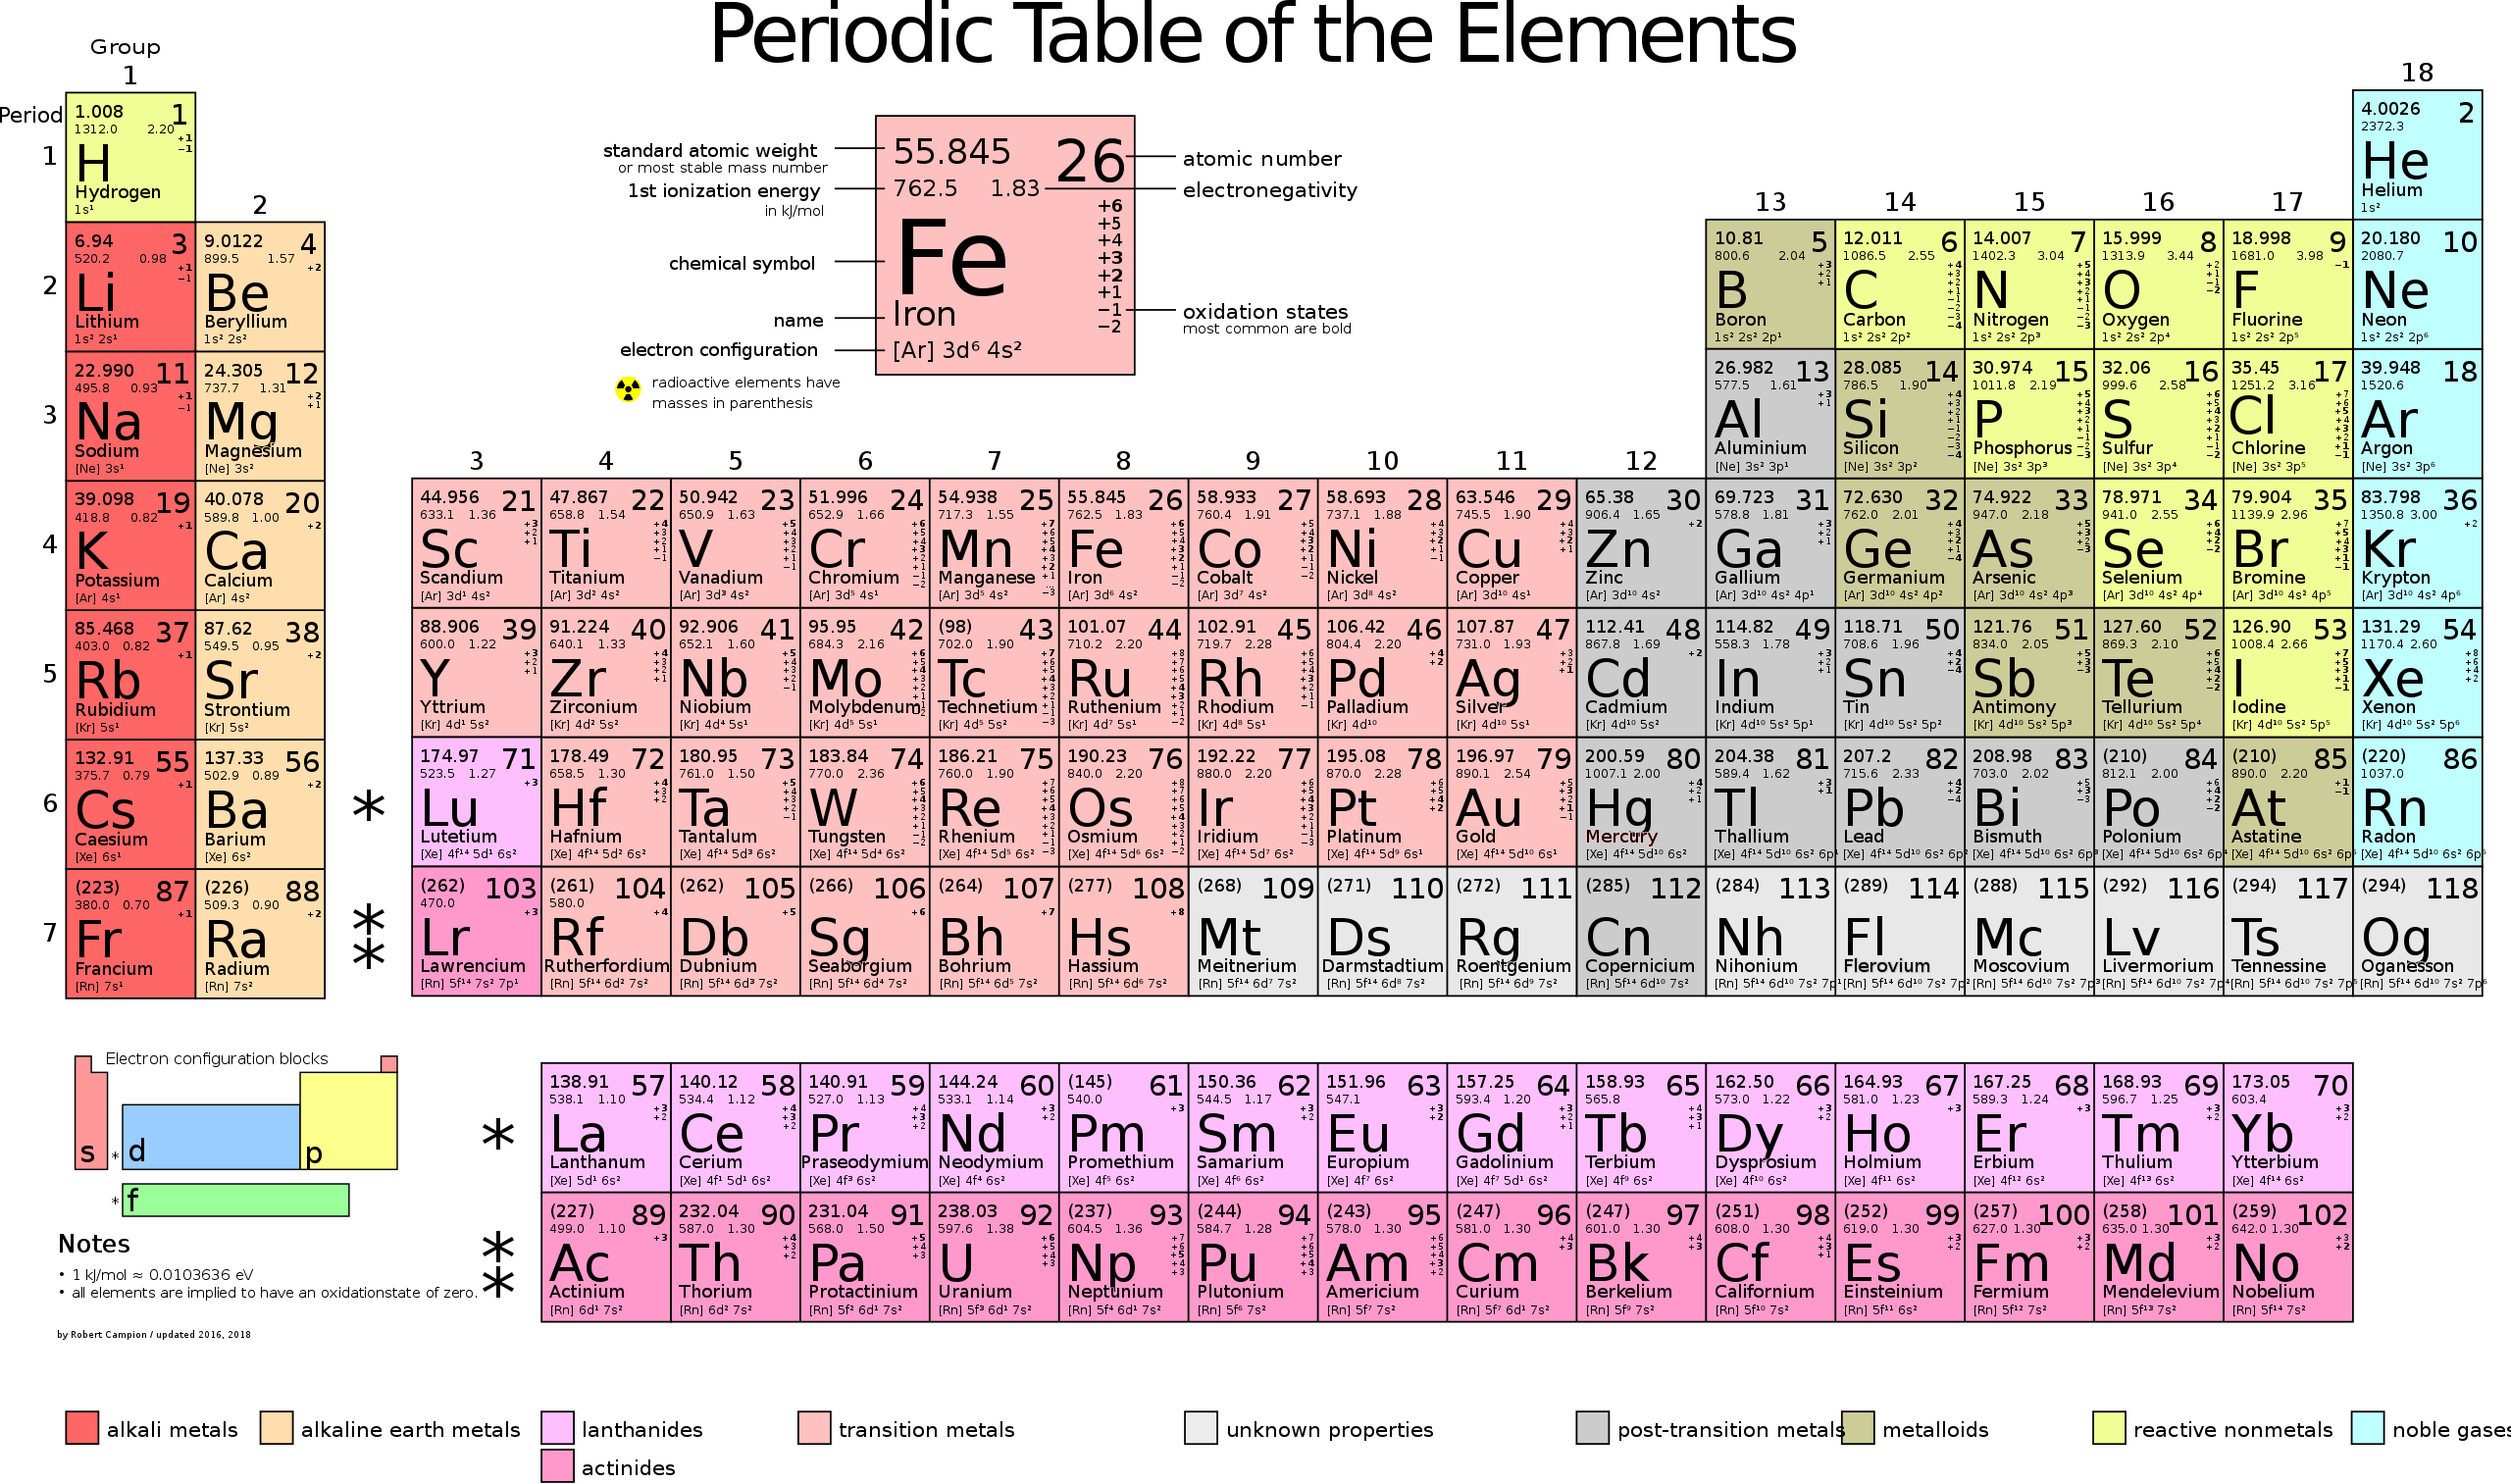
\includegraphics[width=\textwidth]{./chemistry/imgs/ptoe.png}
\\
Relative atomic mass (deprecated atomic weight) is ration to the atomic mass unit (amu), see Stoichiometry\\
Going down the table increases the radii of the atom (more shells).\\
Going right decreases the radii because more protons = more force inward.

\begin{description}
    \item[Dmitri Mendeleev] The Father of the Periodic Table.
    \item[Protons] atom type/number
    \item[neutron] stable / instable (isotopes)
    \item[electron] negative (cation + \& anion-, ions)
    \item[Alkali Metals] Also known as group IA
    \begin{description} 
        \item[] Very reactive, malleable, ductile, conductors
        \item[] Can explode when exposed to water (especially Cesium and Francium)
        \item[] Stored in inert gas or oil
    \end{description}
    \item[Alkaline Earth Metals] Also known as group IIA
    \begin{description} 
        \item[] Smaller atomic radii than alkali metals
        \item[] Readily form divalent cations
    \end{description} 
    \item[Transition Metals] Side group
    \begin{description} 
        \item[] Fairly unreactive, malleable
        \item[] High melting point, conductive
        \item[] Wide oxidation range
        \item[] Low ionization energy
    \end{description}
    \item[Halogens] Also known as group VIIA
    \begin{description}
        \item[] Highly reactive with alkali and alkaline earth metals
    \end{description}
    \item[Nobel gas] Also known as group VIIIA
    \begin{description}
        \item[] Non-reactive
        \item[] High ionization energy
    \end{description}
\end{description}
%
Ionization energy increases up and right\\ 
Electron affinity increases up and right (except noble gas)(how easy to gain an extra electron)
